\documentclass[a4paper,11pt]{article} %, landscape report

\usepackage[T1]{fontenc}
\usepackage[utf8x]{inputenc}

%Selon les goûts: times palatino bookman newcent chancery helvet avant fourier kpfonts cmbright
%\usepackage{avant}

%\usepackage[hmargin=2cm,vmargin=2cm]{geometry}
%\usepackage{multicol}
%\setlength{\columnsep}{1cm}
\usepackage{ragged2e}% for \justifiy

\usepackage{graphicx}
\usepackage{xcolor}
\usepackage{multicol}\setlength{\columnsep}{1cm}

\usepackage{amsmath,amssymb,amsfonts,makeidx}
\usepackage{stmaryrd}% crochets «intervalles d'entiers»
%\newcommand{\B}{\mathbb{B}}
\usepackage{tikz}
\newcommand{\e}{\text{e}}

\usepackage{lscape}

\newcommand{\vesp}{\vspace*{0.2em}}
\newcommand{\VESP}{\vspace*{0.8em}}
\newcommand{\ttt}[1]{\texttt{#1}}
\newcommand{\code}[1]{\colorbox{gray!15}{\texttt{#1}}}
\newcommand{\rem}[1]{\colorbox{yellow}{\textbf{#1}}}
\newcommand{\evid}[1]{\colorbox{blue!10}{\textbf{#1}}}

\usepackage{hyperref}
\hypersetup{colorlinks=true,
            linkcolor=violet,
            urlcolor=teal,
            citecolor=olive,
            }
\newcommand{\www}[2]{\href{#1}{\nolinkurl{#2}}}
%black, blue, brown, cyan, darkgray, gray, green, lightgray, lime, magenta, olive, orange, pink, purple, red, teal, violet, white, yellow
%\urlstyle{same}% Pas stylés \og URL

%\usepackage[nosort]{cite}

%\usepackage{minted}
%\usemintedstyle{%friendly, %colorful, %autumn
%    breaklines, fontfamily=courier,%helvetica,%tt,
%    bgcolor=gray!10,
%    %framesep=2mm,
%    %fontsize=\large,
%    %frame=lines,%single,
%    numbers=none,%left,
%    autogobble, mathescape, texcomments,
%    %stepnumber=2,
%    escapeinside=\%
%}
%% Inline
%\newcommand{\Py}[1]{\mintinline[bgcolor=gray!15]{python}{#1}}
%\newcommand{\BPy}[1]{\textbf{\Py{#1}}}
%\newcommand{\SerreCode}{\vspace*{-0.8em}}
\newcommand{\Py}[1]{\colorbox{gray!20}{\texttt{#1}}}

%\newcommand{\1}{\textcircled{\small 1}}
%\newcommand{\2}{\textcircled{\small 2}}
\setlength{\parskip}{0.2em}
%\setlength{\parindent}{0ex}

\usepackage[french]{babel} \frenchbsetup{StandardLists=true}
\usepackage[autolanguage]{numprint}
\DecimalMathComma

\AddThinSpaceBeforeFootnotes
\FrenchFootnotes

% =================================================================================================
\title{\emph{Résumé de}\\\textbf{Deep Learning with Differential Privacy}\\\small{arXiv:1607.001333}}
%\author{Jean-Marc Gervais\\[0.6em]
%Encadré par M. Jean-François Couchot\\
%\small Institut FEMTO-ST, UMR 6174 CNRS -- DISC Équipe AND}
\date{}

\begin{document}%\setlength\parindent{5mm}
\maketitle
%%
%\section*{\center Notes...\\[1cm]pytorch-dp}
%%
%\thispagestyle{empty}
%\newpage
%%

%\tableofcontents

%\newpage
%%
\section{Vue d'ensemble}
%%
Le \emph{Machine Learning} (ML) à base de réseaux neuronaux repose sur l'exploitation de données d'apprentissage nombreuses, issues du monde réel et qui peuvent donc contenir des informations sensibles. Ces dernières ne devraient pas être récupérables à partir du modèle construit par le réseau de neurones. L'article date de fin octobre $2\,016$. Il analyse les techniques qui permettent de le garantir dans une certaine mesure et propose un outil pour comptabiliser le \og budget de confidentialité\fg{} qu'on doit déterminer au départ et qui est consommé ensuite par l'utilisation des données d'entraînement.

La démarche proposée permet une utilisation plus parcimonieuse de ce budget, par rapoort aux approches décrites jusque là. La mémoire utilisée est moindre, grâce à une utilisation de \emph{batches} de plus petite taille. La méthode reste adaptée aux fonctions d'objectif non convexes. La mise en œuvre s'appuie sur le \emph{framework} \ttt{TensoFlow} développé par Google. Elle est illustrée sur les \emph{datasets} publics classiques de catégorisation d'images que sont \ttt{MNIST} ()\emph{reconnaissance de chiffres manuscrits sur des images monochromes} et \ttt{CIFAR-10} (\emph{identification d'objets et d'animaux, sur des images en couleur}).

On peut noter que les applications de ML contiennent déjà fréquemment des éléments qui contribuent au respect de la confidentialité des données d'entraînement. Il s'agit notamment des traitements pour éviter le surentraînement (\emph{overfitting}), sorte d'apprentissage par cœur stupide qui ferait focaliser le modèle sur des détails spécifiques aux exemples donnés pour l'apprentissage, en perdant de vue les caractéristiques réellement discriminantes dans le cas général. Mais même si le fonctionnement interne des réseaux neuronnaux est difficile à expliciter, certains ont montré qu'on pouvait parfois retrouver en partie des informations utilisées pour l'entraînement du modèle, comme des images sur un algorithme de reconnaissance faciale.

Pour rester dans un cadre réaliste, on considère ici un adversaire ayant accès aux réponses du modèle à ses requêtes et qui dispose potentiellement de données et d'une puissance de calcul sans limites. Il sera même censé connaître complètement le mécanisme d'apprentissage, dont ses paramètres. Le cadre de la confidentialité différentielle est parfaitement adapté à cet effet.
%
\subsection{Confidentialité différentielle}
%
Les définitions essentielles sont rappelées: deux bases de données sont dites \evid{adjacentes} quand elles ne diffèrent que d'un unique enregistrement, présent uniquement dans l'une des deux. On dit alors qu'un méchanisme randomisé $\mathcal{M}: \mathcal{D}\to\mathcal{R}$ garantit la \evid{$(\varepsilon, \delta)$-DP} (pour \emph{Differential Privacy}, confidentialité différentielle), si quelles que soient les entrées $d$ et $d'$ adjacentes de $\mathcal{D}$ et les parties $S$ et $S'$ de $\mathcal{R}$, on a
\[ \mathbb{P}\left(\mathcal{M}(d) \in S\right)   \leqslant  e^\varepsilon \, \mathbb{P}\left(\mathcal{M}(d) \in S'\right) + \delta\]
Il s'agit déjà d'un relâchement (C. Dwork $2\,006$), de la définition originale de la \og pure\fg{} \evid{$\varepsilon$-DP} (cas où $\delta=0$): la valeur de relâchement $\delta$, typiquement inférieure à $\frac{1}{|d|}$, est la probabilité que la garantie de confidentialité différentielle soit mise en défaut. Le nombre $\varepsilon$ peut être interprété comme un \evid{budget de confidentialité}. [Ajout: \emph{cette version relâchée a été introduite pour pouvoir s'adapter à l'ajout d'un bruit qui suit une loi de Gauss plutôt que de Laplace}].

La DP a des propriétés bien utiles dans le contexte du ML: \textbf{compatibilité avec la composition} (l'enchaînement de deux mécanismes, respectivement $(\varepsilon, \delta)$-DP et $(\varepsilon', \delta)$-DP, est $(\varepsilon + \varepsilon', \delta)$-DP), \textbf{confidentialité de groupe} (\emph{dégradation progressive de la confidentialité quand l'effectif augmente}),  la \textbf{robustesse vis à vis des informations auxiliaires} connues par l'adversaire, etc.

La \evid{sensibilité} d'une fonction réelle déterministe sur $\mathcal{D}$, notée $S_f$, est le maximum pour des entrées $d$ et $d'$ adjacentes, de l'écart absolu en sortie $|f(d)-f(')|$. L'ajout à $f$ d'un bruit aléatoire de loi normale centrée d'écart-type $S_f \cdot \sigma$, soit $\mathcal{N}(0,\ S_f^2 \cdot \sigma^2)$, garantit la $(\varepsilon, \delta)$-DP si $\delta \leqslant \frac{4}{5}\exp (-(\sigma\varepsilon)^2/2)$ et $\varepsilon < 1$. Cet exemple montre qu'on dispose d'une infinité de paramétrages optimaux, représentables sur une courbe implicite.
%
\subsection{Deep Learning}
%
Les différentes couches des réseaux \og profonds\fg{} du \emph{Deap Learning} (DL) définissent des fonctions paramétrées associant les sorties aux entrées, comme composées de couches multiples. Ces blocs élémentaires sont des transformations affines, des fonctions non-linéaires simples (souvent ReLU \emph{REctified Linear Unit} qui vaut 0 dans les négatifs et l'identité dans les positifs, ou sigmoïde $\sigma(x) = \frac{1}{1+\exp(-\lambda x)}$).

On définit une fonction d'objectif, ou de perte $\mathcal{L}$ (pour \emph{loss}) qui pénalise l'écart aux résultats attendus, en sortie, pour des données d'entraînement. Plus précisément, $\mathcal{L}(\theta)$ est la moyenne des pertes $\mathcal{L}(\theta, x)$ pour chacune des entrées $x$, sur l'ensemble des données d'entraînement considérées, pour des paramètres $\theta$ donnés. Entraîner le réseau neuronal revient à minimiser au mieux cette quantité, ce qui est difficile dans les réseaux complexes où $\mathcal{L}$ n'est généralement pas convexe.

En pratique on utilise souvent la descente de gradient stochastique (\evid{SGD} \evid{\emph{Stochastic Gradient Descent}}): à chaque étape, on forme un lot $B$ (on utilisera ici l'anglais \emph{batch} pour bien identifier chaque entité sans confusion) d'entrées d'entraînement tirées aléatoirement, sur lesquelles on calcule le gradient moyen $\mathbf{g}_B = \frac{1}{|B|}\sum_{x\in B}\nabla\theta \mathcal{L}(\theta, x)$, qu'on utilise pour mettre à jour les paramètres de $\theta$ (d'un \og pas\fg{} donné, suivant $-\mathbf{g}_B$). TensorFlow automatise les calculs de cette rétropropagation du gradient.

%%
\section{Approche choisie dans l'article}
%%
Ici, la SGD est adaptée pour garantir la DP (version DP-SGD). On explique comment gérer le budget de confidentialité ($\varepsilon$) et configuer les hyperparamètres (\emph{on nomme ainsi ceux de l'algorithme, pour les distinguer des coefficients calculés par le réseau neuronal et adaptés au fur et à mesure de son apprentissage}).
%
\subsection{Principe de la DP-SGD}
%
Traiter en sortie le réseau vu comme \og boite noire\fg{} à l'issue de son entraînement pour en garantir la confidentialité demande d'ajouter trop de bruit pour conserver un résultat utilisable, car la DP impose de considérer le pire cas. Une approche plus sophistiquée (\emph{pas nouvelle, mais affinée notamment pour la comptabilité du budget de confidentialité}) est adoptée ici:  intervenir à chaque phase du calcul du gradient.

Concrètement, dans l'\textbf{algorithme 1}, à chaque étape (ou temps $t$) on échantillonne parmi les données d'entraînement un \emph{batch} aléatoire $L_t$ (avec une probabilité de $L/N$, où $L$ est la taille de ces groupes et $N$ celle des données), puis dessus:
\begin{itemize}
   \item
   Sur chacun des éléments $x_i$
   \begin{itemize}
       \item
       On calcule le gradient de la fonction de perte $\mathbf{g}_t(x_i) = \nabla_{\theta_t } \mathcal{L}(\theta)$
       \item
       On le remet à l'échelle si besoin, de manière à limiter sa norme  euclidienne $\ell_2$ au seuil maximal $C$ fixé (c'est l'un des hyper-paramètres). Notons $\bar{\mathbf{g}}_t(x_i)$ le résultat. Remarquons que si cette étape d'écrêtage ou \emph{clipping}  est classique en SGD standard, elle s'exerce alors généralement sur la valeur moyenne calculée ci-après, plutôt que sur  chacune des données comme ici où l'on doit limiter leur influence individuelle pour pouvoir garantir la confidentialité différentielle.
       \item
       On ajoute un bruit aléatoire qui suit la loi normale centrée d'écart-type $\sigma C$ suivant chaque dimension, soit  $\mathcal{N}(0,\, \sigma^2 C^2 \mathbf{I})$. La justification de la DP s'appuie sur la majoration de la norme $\ell_2$ du gradient garantie par l'étape prédédente.
   \end{itemize}
   \item
   On calcule la moyenne $\tilde{\mathbf{g}}$ de ces gradients individuels bruités.\rem{pas clair: bruit sur chaque ?}
   \item
   On ajuste les paramètres comme pour une SGD classique, compte tenu du taux d'apprentissage $\eta_t>0$, autrement dit : $\theta_{t+1}$ prend la valeur $\theta_t - \eta_t \tilde{\mathbf{g}}_t$.
\end{itemize}

Dans le cas d'un réseau multi-couches, chacune peut être traitée individuellement, avec ses propres valeurs de $C$ et de $\sigma$. De plus, ces dernières au temps $t+1$ peuvent varier en fonction de l'étape $t$ (pour les exemples donnés, on restera cependant sur des réglages constants pour $C$ et $\sigma$).

Une distinction peut être faite entre un \evid{\emph{lot}} (\emph{in english}), groupe de taille $L$ de données utilisées pour calculer la moyenne empirique du gradient et le \evid{\emph{batch}} correspondant au groupement habituel pour le calcul de gradient. Ainsi, pour limiter la consommation de mémoire, on pourrait choisir une taille de \emph{batch} bien inférieure à $L$, sur lequels on effectuerait les calculs, et ajouter le bruit sur le lot constitué de l'ensemble des \emph{batches}. En pratique, par souci d'efficacité on permute aléatoirement les entrées, puis on partitionne. Mais pour les raisonnements, on considère que chaque exemple est tiré avec une probabilité de $q=L/N$, $N$ étant la taille du \emph{dataset} d'entraînement.
%
\subsection{Comptabilité du budget de confidentialité plus en détails}
%
La compatibilité avec la composition permet les calculs nécessaires : à chaque utilisation de données d'entraînement, on en consomme une partie qui se cumule avec les autres \og dépenses \fg{}. En choisissant $\sigma = \sqrt{2\log \frac{1,25}{\delta}}/\varepsilon$, chaque étape est $(\varepsilon,\,\delta$)-DP vis à vis du \emph{lot}, lui-même échantillonné sur la base complète, donc $(O(q\varepsilon),\,q\delta$)-DP par rapport à l'ensemble des données d'entraînement, avec $\varepsilon < 1$ (\emph{cf. théorème d'amplification, Kasiviswanathan $2\,011$}).
configure
Pour améliorer le résultat obtenu avec le théorème fort de composition, meilleur résultat jusque là, mais qui ne tient pas compte la distribution du bruit ajouté, la nouveauté est l'utilisation du \evid{\emph{moments accountant}} dans de cadre de la DP-SGD (et plus simplement la SGD standard). On prouve qu'en choisissant convenablement le niveau de bruit et le seuil de \emph{clipping}, la DP-SGD est $(O(q\varepsilon\sqrt{T}), \,\delta))$-DP où $T$ est le nombre de cycles, d'\emph{epoch}. Le gain est d'un facteur $\sqrt{log(1/\delta)}$ sur $\varepsilon$ et de $Tq$ sur $\delta$ par rapport au théorème fort de composition.

Au final, le \textbf{théorème 1} montre qu'il existe des constantes $c_1$ et $c_2$ telles qu'étant donnés $q=L/N$ le taux d'échantillonnage et $T$ le nombre d'étapes, l'algorithme précédent est $(\varepsilon, \delta)$-DP pour tout $\varepsilon < c_1 q^2 T$ et tout $\delta > 0$, si l'on choisit
\[ \sigma \geqslant c_2 \dfrac{q\sqrt{T \log(1/\delta)}}{\varepsilon} \]
Le gain théorique par rapport au théorème fort de composition est vérifié en pratique.

L'élément comptable \emph{moments accountant} est conçu spécifiquement pour suivre le budget de confidentialité, de manière \og serrée\fg{}. La perte de confidentialité ou \evid{\emph{privacy loss}}, pour un mécanisme $\mathcal{M}$, une entrée auxilaire $\text{aux}$ (qui sera typiquement constitudée des sorties aux étapes précédentes, dans les enchaînements d'appels), des bases adjacentes $d$ et $d'$ et une sortie $o$, est définie par
\[c(o; \mathcal{M},\text{aux}, d, d')=\log\frac{\mathbb{P}[\mathcal{M}(\text{aux}, d)=o]}{\mathbb{P}[\mathcal{M}(\text{aux}, d')=o]} \]
On définit alors le \evid{$\lambda^\text{e}$ moment} $\alpha_\mathcal{M}(\lambda; \text{aux}, d, d')$ comme le logarithme de la fonction génératrice des moments, en $\lambda$, soit $\log \mathbb{E}_{0\sim\mathcal{M}(\text{aux},d)} [\exp(\lambda\, c(o; \mathcal{M},\text{aux}, d, d')]$ et on utilise
\[ \alpha_\mathcal{M}(\lambda)=\max_{\text{aux}, d, d'} \alpha_\mathcal{M}(\lambda; \text{aux}, d, d') \]
 (où la maximum est pris sur toutes les entrées auxiliaures $\text{aux}$ et toute les bases adjacentes $d$ et $d'$) pour la garantie de confidentialité. Le \textbf{théorème 2} montre alors que si l'on enchaîne une séquence (\og adaptative\fg{}, où chaque phase peut utiliser sur les sorties des précédentes) de mécanismes $\mathcal{M}_i$, on a
 \[\alpha_\mathcal{M}(\lambda) \leqslant \sum \alpha_{\mathcal{M}_i}(\lambda)\]
 \centering(compatibilité avec la composition)\justify
  et pour tout $\varepsilon > 0$, le mécanisme $\mathcal{M}$ est $(\varepsilon,\, \delta)$-DP pour
 \[ \delta = \min_\lambda\   \exp(\alpha_\mathcal{M} (\lambda)-\lambda \varepsilon) \]
\centering(majoration de la queue de la distribution)\justify

Il suffit donc de majorer $\alpha_{\mathcal{M}_i}(\lambda)$ à chaque étape$^*$ pour borner le moment global, puis d'utiliser la seconde partie du théorème pour convertir cela en garantie de $(\varepsilon,\, \delta)$-DP. La principale difficulté reste au niveau de la première phase (\emph{cf. }*).
Dans le cas du mécanisme gaussien avec échantillonnage aléatoire de probabilité $q$, on montre que
\[ \alpha(\lambda) \leqslant q^2 \lambda (\lambda+1) / (1-q)\lambda^2 + O(q^3/\sigma^3)  \]
%%% Explication à compléter, reportées plus bas...
%note $\mu_0$ et $\mu_1$ les densités des lois normales centrées respectivement en $0$ et$1$ et d'écart-type $\sigma$. Puis on pose $\mu = (1-q)\mu_0 + q \mu_1$.
%
\subsection{Réglage des hyper-paramètres}
%
La justesse (\emph{accuracy}) du modèle s'avère plus sensible aux paramètres d'entraînement comme la taille du \emph{batch} et le niveau de bruit qu'à la structure du réseau. En particulier pour les fonctions d'objectif non convexes, il est préférable de choisir une taille de \emph{batch} supérieure à 1, contrairement aux cas convexes, sans toutefois être trop importante pour préserver la confidentialité (\emph{cf.} théorème 1), disons du même ordre de grandeur que le nombre attendu d'\emph{epochs}.

En DP-SGD, le taux d'apprentissage n'aura pas à être progressivement diminué jusqu'à une très faible valeur. On constate qu'on a intérêt à partir d'un niveau assez grand, qui diminue linéairement sur quelques \emph{epochs}, puis reste constant ensuite.

%%
\section{Expérimentations}
%%

[\emph{Note: comme c'est TensoFlow qui est utilisé ici, on détaillera moins, tâchant plutôt de repérer ce qui pourrait avoir été repris dans pytorch-dp..}]

On retrouve les phases de \emph{sanitization} (\emph{clipping}) du gradient, puis d'ajout de bruit avec suivi du budget de confidentialité alloué. Pour la première, on retrouve le même module \ttt{per\_example\_gradient} que dans pytorch, qui effectue ce calcul efficacement (sur des couches cachées classiques, mais pas à ce stade sur celles de convolution\\ \rem{à comparer donc avec \og notre\fg{} solution qui devrait les prendre en charge...})\\

Le \emph{moments accountant} est utilisé pour le second point. On peut traduire à tout moment le résultat en $(\varepsilon, \delta)$-DP, plus facilement interprétable. Le $\alpha(\lambda)$ est calculé à partir de
$\mu_0$ et $\mu_1$, les densités des lois normales centrées respectivement en $0$ et$1$ et d'écart-type $\sigma$. On pose $\mu = (1-q)\mu_0 + q \mu_1$ et $\alpha(\lambda)$ vaut $\log \max(E_1, E_2)$ où $E_1 = \mathbb{E}_{z\sim\mu_0}[(\mu_0(z)/\mu(z))^\lambda]$ et $E_2 = \mathbb{E}_{z\sim\mu}[(\mu(z)/\mu_0(z))^\lambda]$.
Pour éviter de faciliter une attaque basée sur l'analyse de l'adaptation dynamique des paramètres, ces derniers sont ici fixés \emph{a priori}.

%
\subsection{DP-PCA}
%

Un prétraitement des données par analyse en composantes principales (PCA) est intéressante pour optimiser l'utilisabilité des données d'entraînement. Pour la rendre DP-compatible, ici, une technique connue est reprise (échantillonnage aléatoire, transformation en vecteurs-lignes $\ell_2$-normalisés pour former une matrice $A$, puis ajout de bruit gaussien à la matrice de covariance $A^TA$ avant la PCA sur cette dernière).
Cela consomme une part du budget de confidentialité, mais semble intéressant étant donné le gain de qualité sur le modèle et la réduction du temps d'entraînement induite.

<<<<<<< HEAD

%%
\section{Expérimentations}
%%
L'idée est notamment de comparer la consommation du budget de confidentialité obtenue, par rapport à l'application du théorème for de composition. Les paramètres sont calculé en fonction de
\begin{itemize}
    \item
    $\sigma$ le niveau de bruit.
    \item
    $q=L/N$ le ratio d'échantillonnage: une \emph{epoch} consiste donc en $1/q$ \emph{batches}.
    \item
    $E$ le nombre d'\emph{epochs} (d'où $E/q$ étapes).
\end{itemize}
On fixe $\delta = 10^{-5}$, et on calcule $\varepsilon$ en fonction de $E$, avec $q=0,01$ et $\sigma = 4$. Grossièrement, le gain est de l'ordre de $10$ sur $\varepsilon$ pour quelques centaines d'\emph{epochs}.
%
\subsection{MNIST}
%
Le réseau neuronal est composé d'une PCA en $60$ dimensions (on note $\sigma_p$ le bruit associé pour la DP), suivi d'une couche cachée unique à $1\,000$ unités avec ReLU (bruit $sigma$; les résultats sont meilleurs qu'avec $2$ couches cachées), en utilisant une taille des \emph{lots} de $600$, Le \emph{clipping} du gradient est effectué à la norme $4$ pour chaque couche. [\emph{L'architecture choisie est donc assez différente de celle de l'exemple MNIST choisi pour pytorch-dp}].

Trois niveaux de bruit sont comparés, $(\sigma, \sigma_p)$ vallant $(2; 4)$, $(4; 7)$ puis $(8; 16)$.

Le taux d'apprentissage est initialisé à $0,1$. Il décropoît linéairement jusqu'à $0,052$ sur $10$ \emph{epochs} puis reste constant.
=======
%%
\subsection{MNIST}
%%


\subsection{CIFAR-10}
>>>>>>> f6ddaf29a68888847d4998ad4f41879b7f30bf4f




%
\subsection{CIFAR-10}
%
%

%\begin{center}
  %  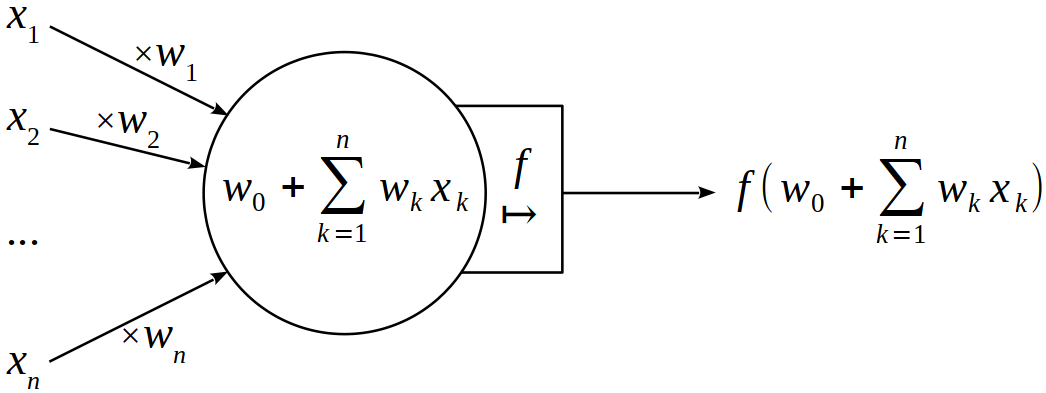
\includegraphics[width=0.7\linewidth]{neurone.png}
%\end{center}
\begin{itemize}
    \item
\end{itemize}

\end{document}